\section{Lecture 5: LSZ Reduction }
We want to compute the S-matrix to computable quantities. From the Lehmann-Kallen representation of the propagator, we have that under mild assumptions for our theory, the single particle state of the free theory survives in the interacting theory (with a mass gap). The only potential modifications are:
\begin{enumerate}
    \item A shift from the bare to the physical mass. Non-trivial connection between the mass parameter in the Lagrangian and the physically measured mass.

    \item An overall shift in the normalisation
\end{enumerate}  
 \begin{equation}
        \mel{k}{\phi_{\text{free}}(x) }{0} = Z^{1/2}  \mel{k}{\phi_{\text{full theory}}(x) }{\Omega} 
    \end{equation} where $\bra{k}$ is the single particle state in the free theory, $\phi_{free}$ is the field in free theory and $\ket{0}$ is the vacuum in the free theory. Here $Z^{1/2}$ is the wavefunction normalisation, And $\bra{k}$ and $\ket{\Omega}$ are the eigenstates of the full theory. One find that $0 \leq z < 1$ in the interacting theory and $z = 1$ in the free theory.

    We will simply state the LSZ reduction theorem
    \begin{align}
        & \expval{ p_1 \dots p_m; \text{out}  | k_1 \dots k_l ; \text{in}   }   =  \int d^{n+1} x_1 \dots d^{n+1} x_m d^{n+1} y_1 \dots d^{n+1} y_{l} \nonumber\\
        & e^{i \sum_{i=1}^{m}  p_i \cdot x_i } e^{-i \sum_{j=1}^{l}  k_j \cdot y_j } (i)^{m+l} \Pi_{i=1}^{m} (\Box_{x_i}  + m_{\text{physical}}^{2}) \Pi_{j=1}^{l} (\Box_{y_j}   + m_{\text{physical}}^{2}) \nonumber\\
        & \mel{\Omega}{ T\{  \phi'(x_1) \dots \phi'(x_m)\phi'(y_1) \dots \phi'(y_l)  
 \}  }{\Omega} \nonumber\\
 & = \Pi_{i=1}^{m} \frac{p_{i}^{2} - m_{\text{physical}}^{2} }{i}\Pi_{j=1}^{l} \frac{k_{j}^{2} - m_{\text{physical}}^{2} }{i} \tilde{G}' (p_1 \dots p_m; k_1 \dots k_l)
    \end{align}
where 
\begin{align}
    \tilde{G}' (p_1 \dots p_m; k_1 \dots k_l) =  \int d^{n+1} x_1 \dots d^{n+1} x_m d^{n+1} y_1 \dots d^{n+1} y_{l}e^{i \sum_{i=1}^{m}  p_i \cdot x_i } e^{-i \sum_{j=1}^{l}  k_j \cdot y_j } G'(x_1, \dots x_m ; y_1 \dots y_l)
\end{align}
where
\begin{equation}
    G'(x_1, \dots x_m ; y_1 \dots y_l) = \mel{\Omega}{ T\{  \phi'(x_1) \dots \phi'(x_m)\phi'(y_1) \dots \phi'(y_l)  
 \}  }{\Omega}
\end{equation}
is the $m+l$ point "renormalised" Green function.
\begin{figure}[htp]
    \centering
    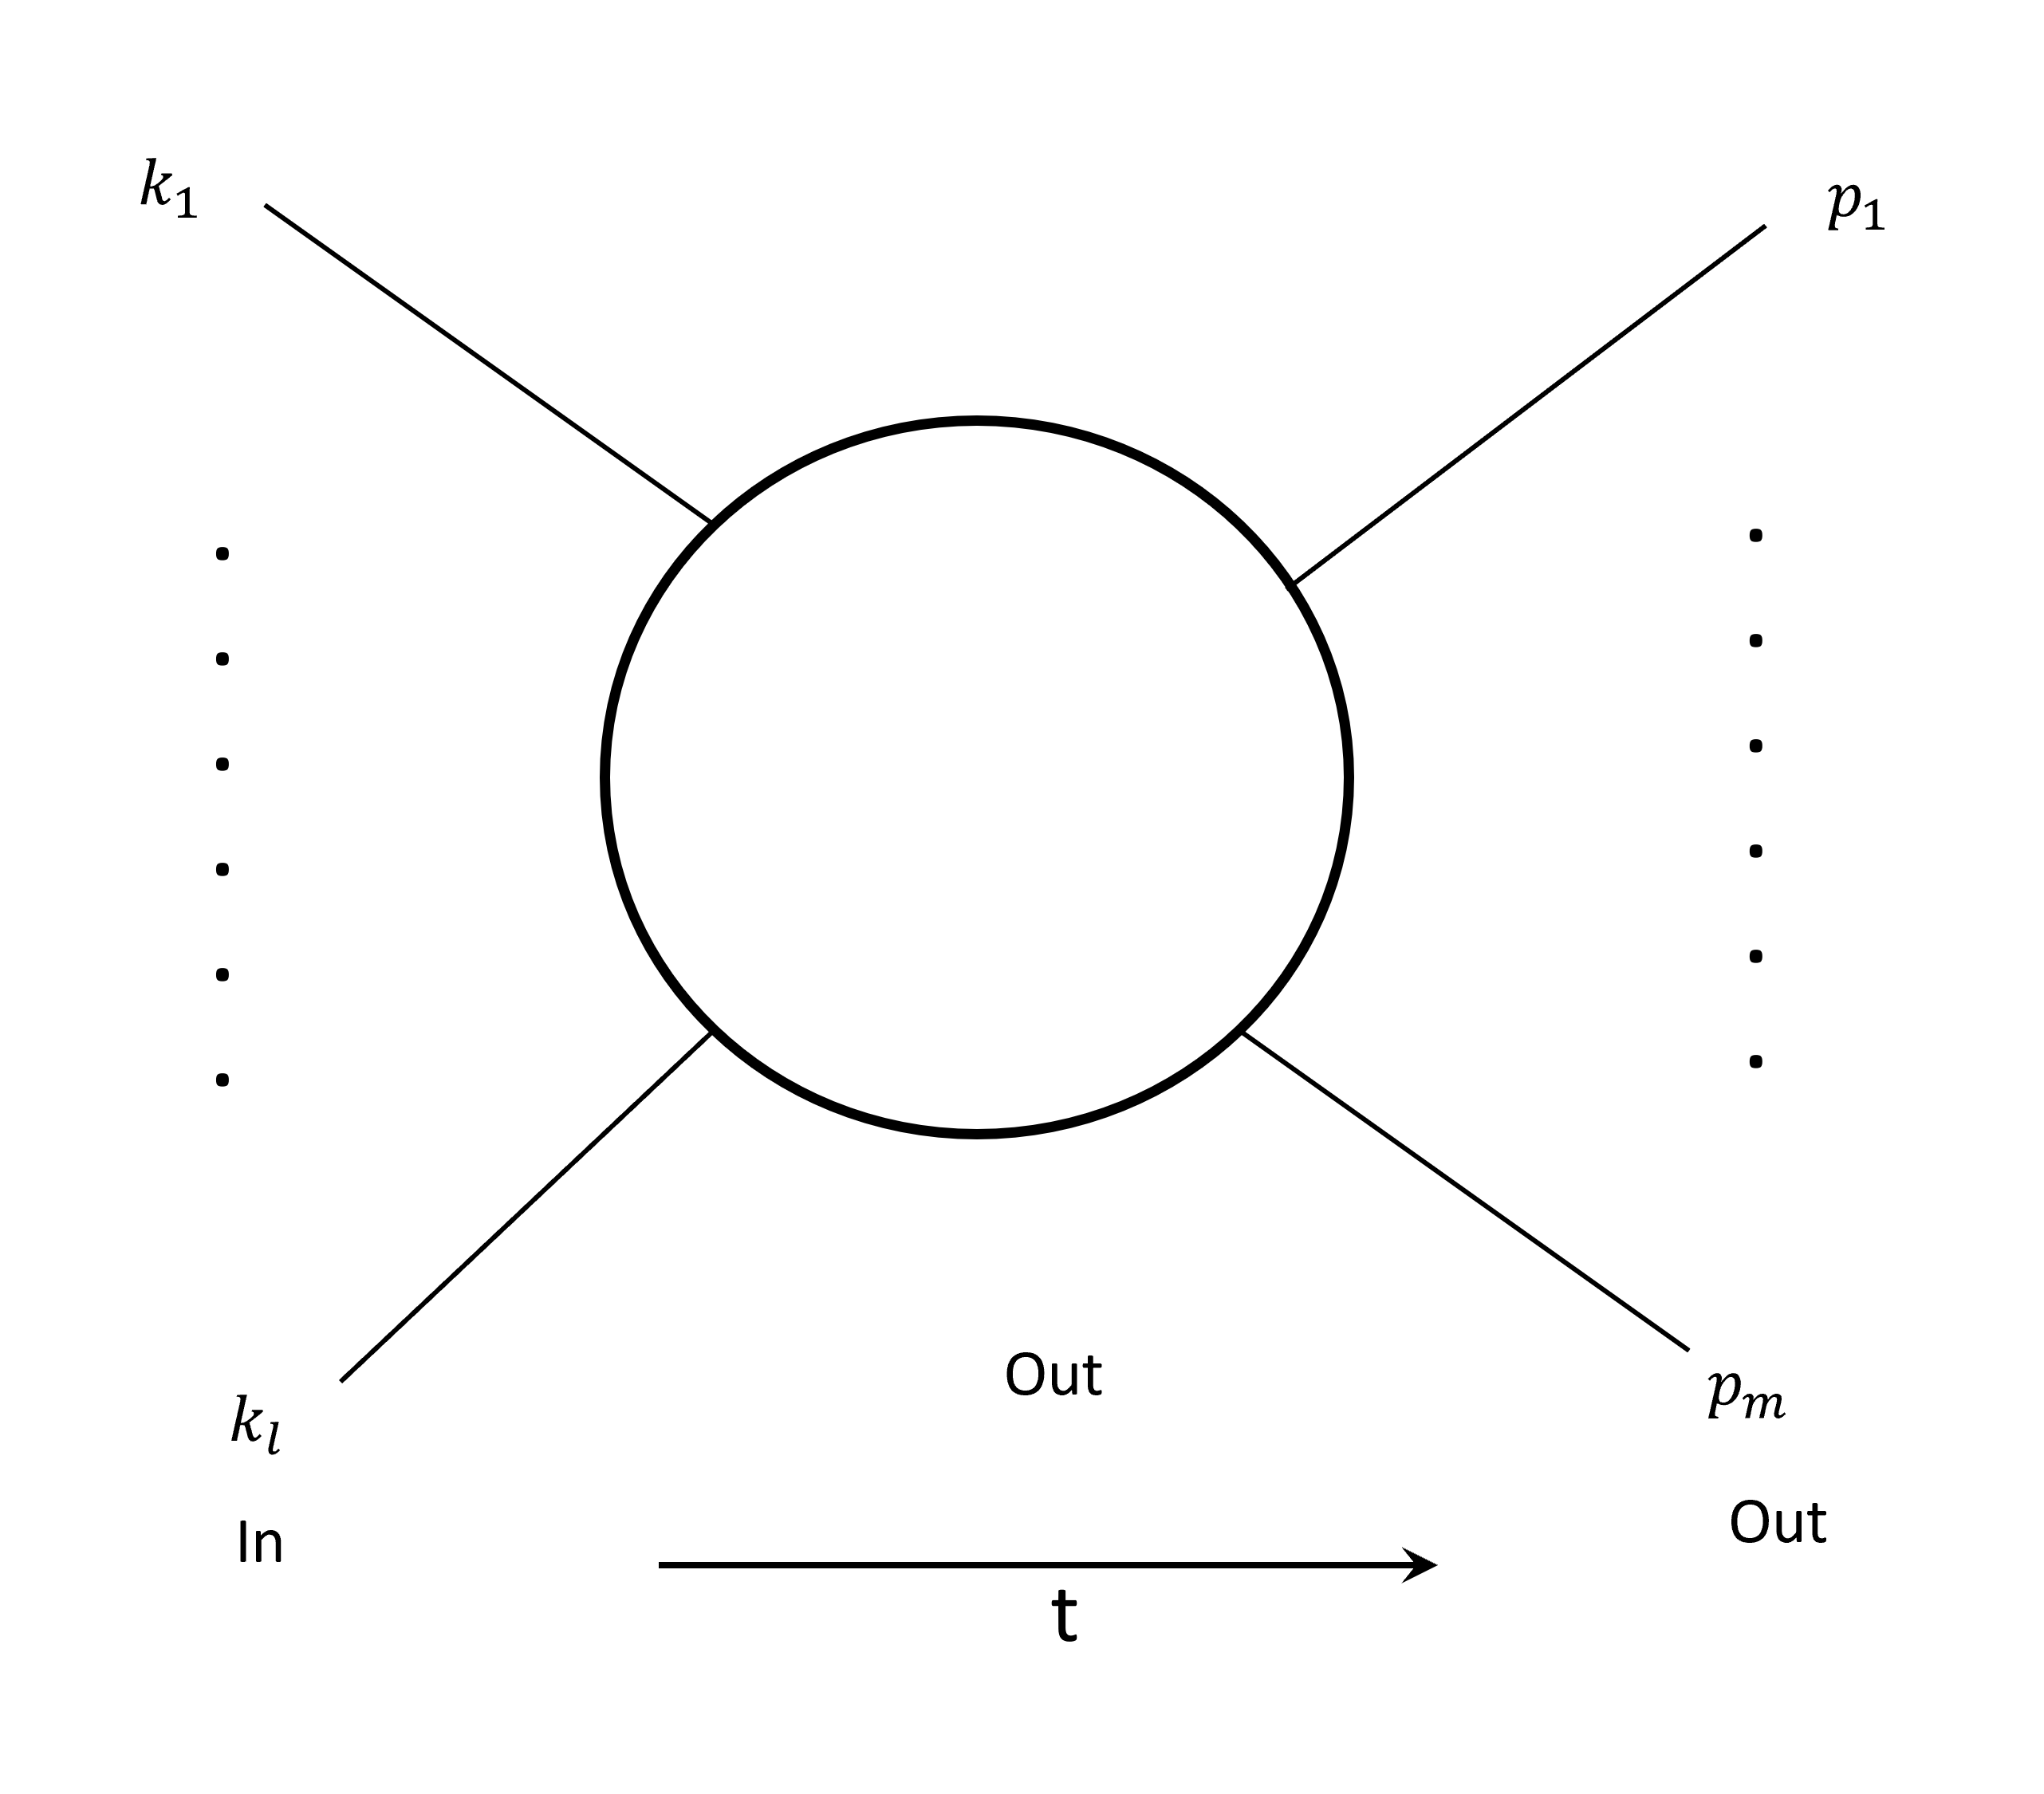
\includegraphics[width = 5cm]{Illustrations/Picture1.png}
    \label{fig:enter-label}
\end{figure}

and 
\begin{equation}
    \frac{p_{i}^2 - m_{\text{physical}}^2}{i} = \left( \frac{i}{p_{i}^{2} -m_{\text{physical}}^{2} }   \right)^{-1}
\end{equation}
is the inverse momentum space propagator; inverse of $K-G$ operator $\Box + m^2$. We have put quotations around renormalised because the Greens Function is associated with the renormalised field $\phi'$, but the definition of $\phi'$ may not exactly correspond with the particular renormalisation scheme chosen for the problem. In particular $\phi'(x)$ is defined such that
\begin{enumerate}
    \item $\mel{\Omega}{\phi'(x)}{\Omega} = 0$
i.e. $\phi'(x)$ has zero VEV.
\item $$\mel{k}{\phi'(x)}{\Omega} = e^{ik\cdot x}$$

\end{enumerate}
Conditions $1, 2$ corresponds with what is called "on shell (os)" renormalisation; i.e. 
\begin{equation}
    \phi'(x) = \phi_{r, os} (x)
\end{equation}
Note that $\phi'(x)$ does not correspond to $\mu S$ or $\bar{\mu} S$ renormalisation scheme, $\phi'(x) \neq \phi_{r, \mu S} (x)   \neq \phi_{r, \bar{\mu}S }$


\subsection{Gell-Mann-Low theorem}

We seek a connection between the renormalised GF in the full theory $\mel{\Omega}{T\{ \phi'(x_1) \dots  \}}{\Omega}$ to something computable (order by order). This connection is provided by the Gell-L theorem.

The full Gell-Mann Low theorem is a statement about adiabatic invariance: 
\begin{equation}
    \hat{H}_{\epsilon} (t) \equiv \hat{H}_{0} + e^{-\epsilon |t|} g \hat{V}
\end{equation}
where $\hat{H}_0$ is the unperturbed Hamiltonian. The exponential corresponds to the adiabatic turning on/off of the interaction. Finally we have $g$ which is the interaction strength which is assumed to be small, it will be our expansion parameter. Here $\hat{V}$ is the interaction. Note that $\hat{H}_0$ and $\hat{V}$ wil be composed of our fields $\phi(x)$, and thus have full spacetime dependence. The point here is that states "evolve into themselves", eg. $\ket{0} \to \ket{\Omega}$ due to $\ket{k} \to \ket{k}$ the adiabatic turning on/off. 

Assuming that we have solved the theory associated with $\hat{H}_0$ and we are interested in the theory $\hat{H}$ where $\hat{H}$ is not too different from $\hat{H}_0$. Lets assume that $\hat{H}_0$ has a mass gap that survives in $\hat{H}$. Sicne we have fully solved $\hat{H}_0$ by assumption, we have a decomposition of unity, 
\begin{equation}
    \hat{\mathds{1}} = \ket{0}\bra{0} + \sumint \ket{l_n} \bra{l_n}
\end{equation}
where $\hat{H}_0 \ket{0} = E_0 (0)$ (strictly) and all $E_n > E_0$, where $E_n$ is the eigen-energy of an eigenstate of $\hat{H}_0$ other than $E_0$, as we have assumed a mass gap. 

Even though we haven't fully solved $\hat{H}$, we still have a decomposition of unity by L-K: 
\begin{equation}
    \hat{\mathds{1}} = \ket{\Omega} \bra{\Omega} + \sumint \ket{\lambda_n} \bra{\lambda_n} 
\end{equation}
where $\hat{H}\ket{\Omega} E_{\Omega} \ket{\Omega}$ and all $E_V > E_{\Omega}$ ,where $E_{V}$ is the eigenvalue of the full theory $\hat{H}$ other than $E_{\Omega}$ , since we have assumed the mass gap survived.

Lets now define the interaction picture. The interaction (or intermediate) picture is between the Schrodinger and Heisenberg pictures. The idea is to  first evolve using the full Hamiltonian $\hat{H}$, then un-evolve using $\hat{H}_0$. The IP is generally useful for performing order by order calculations when $\hat{H}$ is not too different from $\hat{H}_0$ and we have fully solved $\hat{H}_0$.  We thus define the interaction picture time evolution operator as
\begin{equation}
    U_I (t, t_0) \equiv \underbrace{U_{H_0}^{-1} (t, t_0)}_\text{Free Hamiltonian} \underbrace{U_H (t, t_0)}_\text{Full Hamiltonian}
\end{equation}
Note that we have used $U_{H_0}^{-1}$. Most textbooks use $U_{H_0}^{+}$. For $t, t_0 \in \mathbb{R}, U_{H}^{\dagger} = U^{-1}$ is unitary. The IP operators are defined as
\begin{equation}
    \phi_{H}(x)= U_{I}^{-1} (t, t_0) \phi_I (x) U_{I}(t, t_0)
\end{equation}
As per usual, the Heisenberg and IP operators for $t = t_0$. The IP time evolution operator (TEO) obeys all the usual properties of TEO's:
\begin{align}
    U_{I} (t_0, t_0) & = \mathds{1} \nonumber\\
    U_I (t_2, t_1) U_I (t_1, t_0) & = U_I (t, t_0)\nonumber\\
    U_{I}^{-1} (t_0, t_1) & = U_I (t_1, t_0)
\end{align}
we know that
\begin{equation}
    U_{I}(t_0 , t_1) U_{I}^{-1} (t_0, t_1)  = U_{I}(t_0, t_1) U_I (t_1, t_0) = \mathds{1}
\end{equation}
We need to be careful about what exactly is
\begin{align}
    U_I (z_1, z_0) & = U_{H_0}^{-1} (z_1 , z_0) U_{H} (z_1, z_0) \nonumber\\
    & = U_{H_0} (z_0 , z_1) U_{H} (z_1, z_0)
\end{align}
and 
\begin{align}
    U_{I}^{-1} (z_1, z_0) & = [U_{H_0} (z_0 , z_1) U_{H} (z_1, z_0)]^{-1} \nonumber\\
    & = U_{H}^{-1} (z_1 , z_0) U_{H_0}^{-1} (z_0, z_1) \nonumber\\
    & = U_H (z_0 , z_1) U_{H_0} (z_1, z_0)
\end{align}
Hence $U_{I}^{-1} (z_1, z_0)=  U_{I}(z, z_0) =\mathds{1}$
Lets consider
\begin{align}
    \mel{\Omega}{\phi_H (x)}{\Omega} & = \mel{\Omega}{  U_{I}^{-1} (t, t_0)  \phi_I (x)   U_I (z_1, z_0)  }{\Omega} \nonumber\\
    & = \lim_{\epsilon \to 0} \lim_{T \to \infty}  \mel{\Omega}{  U_{I}^{-1} (t, -T (1-i\epsilon)) \phi_I (x) U_I (t, -T(1 - i\epsilon))   }{\Omega}
\end{align}
Here we going slightly back into the past with an imaginary part. Go back to the infinite past such that $\ket{0}$ adiabatically turns on to $\ket{\Omega}$; connects with asymptotic in states. We insert $\hat{\mathds{1}} = U_{I}^{-1} (T (1-  i\epsilon) , t)  U_{I}( T(1 - i\epsilon) , t)$ to take $\phi_I (x)$ to the asymptotic future. We thus have
\begin{align}
    \mel{\Omega}{\phi_H (x)}{\Omega} = \lim_{\epsilon \to 0} \lim_{T \to \infty}  \mel{\Omega}{  U_{I}^{-1} (t, -T (1-i\epsilon))  U_{I}^{-1} ( T(1 - i\epsilon) , t) U_I (T(1 - i\epsilon) , t) \phi_I (x) U_I (t, -T (1 - i\epsilon))  }{\Omega}
\end{align}

Aside: Consider: 
\begin{align}
    & \lim_{\epsilon \to 0 } \lim_{T \to \infty} [ \ket{\Omega} \bra{\Omega} + \dots ] U_I (T (1 - i\epsilon) , t)) \nonumber\\
    & \lim_{\epsilon \to 0 } \lim_{T \to \infty} [ \ket{\Omega} \bra{\Omega} + \dots ] U_{I}^{-1} (t, T(1 - i\epsilon)) \nonumber\\
    & \lim_{\epsilon \to 0 } \lim_{T \to \infty} [ \ket{\Omega} \bra{\Omega} + \dots ] U_{H} ( T(1 - i\epsilon), t) U_{H_0} (t, T(1 - i\epsilon))  \nonumber\\
        & \lim_{\epsilon \to 0 } \lim_{T \to \infty} [ \ket{\Omega} \bra{\Omega} + \dots ] e^{-iH (T(1-i\epsilon) - t}U_{H_0} (t, T(1 - i\epsilon)) \nonumber\\
        &  \lim_{\epsilon \to 0 } \lim_{T \to \infty}\left[  \ket{\Omega} \bra{\Omega} \underbrace{e^{-iE_{\Omega} 
(T (1-i\epsilon) - t) }}_\text{$\sim e^{-\epsilon E_{\Omega} T}$} + \sumint \ket{\lambda_n} \bra{\lambda_n} \underbrace{e^{-iE_\nu (T (1-i\epsilon) - t)  }}_\text{$\sim e^{-\epsilon} E_\nu T$}  \right]U_{H_0} (t, T(1 - i\epsilon)) \nonumber\\
\end{align}
The quantities in the bracket are eigenstates of the full theory. Recall that $E_\nu > E_{\Omega}$. Parenthetically, what does the tume contour looks like? Time is propagating from $-\infty + i\epsilon$ to $+ \infty -i\epsilon$. 
\begin{align}
    \lim_{\epsilon \to 0 } \lim_{T \to \infty}  [ \ket{\Omega} \bra{\Omega} + \dots  ] U_I (T (1 - i\epsilon) , t)) =  \lim_{\epsilon \to 0 } \lim_{T \to \infty} \ket{\Omega} \bra{\Omega}  U_I (T (1 - i\epsilon) , t))
\end{align}
Therefore
\begin{align}
    \mel{\Omega}{ \phi_H (x) }{\Omega} & = \lim_{\epsilon \to 0 } \lim_{T \to \infty} \mel{\Omega}{ U_{I}^{-1} (t, -T(1 - i\epsilon)) U_{I}^{-1} ( T(1 + i\epsilon)  , t )  }{\Omega} \nonumber\\ & \mel{\Omega}{ U_{I} ( T(1 - i\epsilon) , t) \phi_I (x) U_{I} ( t, -T(1 - i\epsilon) )  }{\Omega} 
\end{align}
Lets try to get $U_{I} ( t, -T(1 - i\epsilon) ) \ket{\Omega} \sim U_I (\dots) \ket{0}  \expval{0|\Omega} $. Consider
\begin{align}
      & \lim_{\epsilon \to 0 } \lim_{T \to \infty} U_{I} ( t, -T(1 - i\epsilon) ) \ket{0}\nonumber\\
      & = \lim_{\epsilon \to 0 } \lim_{T \to \infty} U_{I} ( t, -T(1 - i\epsilon) ) [ \ket{\Omega} \bra{\Omega} + \dots  ]\ket{0}\nonumber\\
      & = \lim_{\epsilon \to 0 } \lim_{T \to \infty} U_{I} ( t, -T(1 - i\epsilon) ) \ket{\Omega} \bra{\Omega} \ket{0}\nonumber\\
      & =  \lim_{\epsilon \to 0 } \lim_{T \to \infty} U_{I} ( t, -T(1 - i\epsilon) ) \ket{\Omega} \nonumber\\
      & = \frac{1}{\expval{\Omega|0}}  \lim_{\epsilon \to 0 } \lim_{T \to \infty} U_{I} ( t, -T(1 - i\epsilon) ) \ket{0}
\end{align}
Hence 
\begin{align}
    \mel{\Omega}{ \phi_H  (x) }{\Omega}  & = \lim_{\epsilon \to 0 } \lim_{T \to \infty} \mel{\Omega}{ U_{I}^{-1} (t, -T(1 - i\epsilon)) U_{I}^{-1} ( T(1 + i\epsilon)  , t )  }{\Omega} \nonumber\\ & \mel{\Omega}{ U_{I} ( T(1 - i\epsilon) , t) \phi_I (x) U_{I} ( t, -T(1 - i\epsilon) )  }{\Omega} \nonumber\\
    & = \lim_{\epsilon \to 0 } \lim_{T \to \infty} \mel{\Omega}{ U_{I}^{-1} (t, -T(1 - i\epsilon)) U_{I}^{-1} ( T(1 + i\epsilon)  , t )  }{\Omega} \nonumber\\
    & \frac{1}{\expval{\Omega|0}}  \mel{\Omega}{U_{I} ( T(1 - i\epsilon) , t) \phi_I (x)  U_I (t, -T (1 - i\epsilon ))  }{0}
\end{align}
Consider 
\begin{equation}
    \lim_{\epsilon \to 0 } \lim_{T \to \infty} \bra{0} U_I (T (1 - i\epsilon), t) = \dots =  \lim_{\epsilon \to 0 } \lim_{T \to \infty} \expval{0|\Omega} \bra{\Omega} U_I (\dots)
\end{equation}
Therefore 
\begin{align}
    \mel{\Omega}{ \phi_H  (x) }{\Omega}  & =
      \lim_{\epsilon \to 0 } \lim_{T \to \infty} \mel{\Omega}{ U_{I}^{-1} (t, -T(1 - i\epsilon)) U_{I}^{-1} ( T(1 + i\epsilon)  , t )  }{\Omega} \nonumber\\
    & \frac{1}{|\expval{\Omega|0}|^2}  \mel{0}{U_{I} ( T(1 - i\epsilon) , t) \phi_I (x)  U_I (t, -T (1 - i\epsilon ))  }{0}
\end{align}
Lets now consider the c-number
\begin{align}
    \mel{\Omega}{ \phi_H  (x) }{\Omega}  & =
      \lim_{\epsilon \to 0 } \lim_{T \to \infty} \mel{\Omega}{ U_{I}^{-1} (t, -T(1 - i\epsilon)) U_{I}^{-1} ( T(1 + i\epsilon)  , t )  }{\Omega} \nonumber\\
      & = \lim_{\epsilon \to 0 } \lim_{T \to \infty} \mel{\Omega}{ e^{-iH (-T (1 - i\epsilon) - t)}  e^{-iH_0 (t + T (1 - i\epsilon) - t)}  }{0} \mel{0}{e^{-iH_0 (T (1 - i\epsilon) - t)}  e^{-iH (t - T (1 - i\epsilon) - t)}}{\Omega} \nonumber\\
      & = \lim_{\epsilon \to 0 } \lim_{T \to \infty} e^{2i T(1 - i\epsilon)  (E_{\Omega}  - E_0) } |\expval{\Omega|0}|^2
\end{align}
Now consider 
\begin{align}
     & \lim_{\epsilon \to 0 } \lim_{T \to \infty} \mel{0}{ U_I (T (1-  i\epsilon)  , -T (1 - i\epsilon) ) }{0} \nonumber\\
     & = \lim_{\epsilon \to 0 } \lim_{T \to \infty} \mel{0}{ U_I (T (1-  i\epsilon)  ,t) U_I( t, -T (1 - i\epsilon) ) }{0} \nonumber\\
     & = \dots \nonumber\\
     &= \lim_{\epsilon \to 0 } \lim_{T \to \infty} e^{2i T(1 - i\epsilon)  (E_{\Omega}  - E_0) } |\expval{\Omega|0}|^2 
\end{align}
Therefore
\begin{align}
     \mel{\Omega}{  \phi_H (x) }{\Omega} & = 
      \lim_{\epsilon \to 0 } \lim_{T \to \infty} e^{2i T(1 - i\epsilon)  (E_{\Omega}  - E_0) }  \cancel{|\expval{\Omega|0}|^2} \frac{1}{\cancel{|\expval{\Omega|0}|^2}}  \mel{0}{U_{I} ( T(1 - i\epsilon) , t) \phi_I (x)  U_I (t, -T (1 - i\epsilon ))  }{0} \nonumber\\
     & =\lim_{\epsilon \to 0 } \lim_{T \to \infty}  |\expval{0|\Omega}|^2 \frac{ \mel{0}{U_{I} ( T(1 - i\epsilon) , t) \phi_I (x)  U_I (t, -T (1 - i\epsilon ))  }{0}}{\mel{0}{ U_I (T (1-  i\epsilon)  , -T (1 - i\epsilon) ) }{0}}
\end{align}
Our claim is that $|\expval{0| \Omega}|^2 = 1$, proof: 
\begin{align}
    1 & = \expval{\Omega | \Omega} \nonumber\\
    &  = \lim_{\epsilon \to 0 } \lim_{T \to \infty} \mel{\Omega}{ U_{I}^{-1} (t, T(1 - i\epsilon)) U_{I}^{-1} ( T(1 + i\epsilon)  , t )  }{\Omega} \nonumber\\
    & = \lim_{\epsilon \to 0 } \lim_{T \to \infty}  \bra{\Omega} [\ket{0} \bra{0} + \dots] e^{-iH_0  (T(1 - i\epsilon) - t) } U_H \dots \nonumber\\
    & = \lim_{\epsilon \to 0 } \lim_{T \to \infty} \expval{\Omega|0} \mel{0}{ U_{I} (t, T(1 - i\epsilon)) U_{I}^{-1} (t,  T(1 - i\epsilon) )  }{\Omega}\nonumber\\
    & = \lim_{\epsilon \to 0 } \lim_{T \to \infty}  |\expval{\Omega| 0}|^2
\end{align}
we can therefore write 
\begin{align}
     \mel{\Omega}{  \phi_H (x) }{\Omega} 
     & =\lim_{\epsilon \to 0 } \lim_{T \to \infty}   \frac{ \mel{0}{U_{I} ( T(1 - i\epsilon) , t) \phi_I (x)  U_I (t, -T (1 - i\epsilon ))  }{0}}{\mel{0}{ U_I (T (1-  i\epsilon)  , -T (1 - i\epsilon) ) }{0}}
\end{align}
and \begin{equation}
    U_I (t, t_0) = T_{\leftarrow} \exp[-i \int_{t_0}^{t}  dt' L_I (t') ]
\end{equation}
therefore
\begin{align}
     \mel{\Omega}{  \phi_H (x) }{\Omega} 
     & =\lim_{\epsilon \to 0 } \lim_{T \to \infty}   \frac{ \mel{0}{  T_{\leftarrow} \left\{ \phi_I (x) \exp[-i \int_{-T (1 - i\epsilon) }^{T(1+i\epsilon)}  dt' L_I (t') ] \right\} }{0}}{\mel{0}{ T_{\leftarrow} \exp[-i \int_{-T (1 - i\epsilon) }^{T(1+i\epsilon)}  dt' L_I (t') ] }{0}}
\end{align}
Hence we have for $n$ fields:
\begin{align}
     \mel{\Omega}{  \phi_H (x_1) \dots \phi_H (x_n) }{\Omega} 
     & =\lim_{\epsilon \to 0 } \lim_{T \to \infty}   \frac{ \mel{0}{  T_{\leftarrow} \left\{ \phi_I (x) \dots \phi_{I} (x_n) \exp[-i \int_{-T (1 - i\epsilon) }^{T(1+i\epsilon)}  dt' L_I (t') ] \right\} }{0}}{\mel{0}{ T_{\leftarrow} \exp[-i \int_{-T (1 - i\epsilon) }^{T(1+i\epsilon)}  dt' L_I (t') ] }{0}}
\end{align}
where 
\begin{align}
    \mel{\Omega}{  \phi_H (x_2)  A_H (x_1) }{\Omega} = \mel{\Omega}{  U_{I}^{-1} (t_2, t_0)  \phi_I (x_2) \underbrace{U_{\mp} (t_{21}, t_0) U_{I}^{-1} (t_1, t_0)}_\text{$  U_I (t_2, t_0) U_I (t_0 , t_1) = U_I (t_2, t_1) $} A_I (x_1) U_I (t_1, t_0)   }{\Omega}
\end{align}






